\documentclass[12pt,letterpaper]{report}
\usepackage{graphicx}
\usepackage{scrextend}
\usepackage{vmargin}
\usepackage{graphicx}
\usepackage{multirow}
\usepackage[utf8]{inputenc}
\usepackage[spanish]{babel}
\usepackage{multicol}
\usepackage{enumerate}
\usepackage{float}
\usepackage{amsmath, amsthm, amssymb, amsfonts}
\usepackage[usenames]{color}
\parindent=0mm
\pagestyle{empty}
\definecolor{miorange}{rgb}{0.91, 0.43, 0.0}
\begin{document}
\setmargins{2.5cm}      
{1.5cm}                     
{2cm}  
{24cm}                    
{10pt}                          
{1cm}                          
{0pt}                             
{2cm}
\begin{flushright}
\today
\end{flushright}
\vspace{-1.75cm}
\section*{Tarea Clase 12}
\subsubsection*{Calcular el valor de x de cada figura utilizando las razones trigonométricas vistas:}
\begin{figure}[H]
\centering
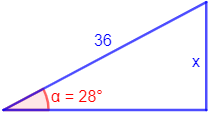
\includegraphics[scale=1]{P1.png}
\caption{Problema}
\end{figure}
La informacion que nos dan es de la la hipotenusa y el cateto opuesto, por lo que se usara seno:
\begin{align*}
    Sen(28)&=\frac{x}{36}\\
    x&=36sen(28)
\end{align*}
\begin{figure}[H]
\centering
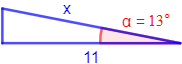
\includegraphics[scale=1]{P2.png}
\caption{Problema}
\end{figure}
Tenemos la hipotenusa y el cateto adyacente, por lo que se usara coseno:
\begin{align*}
    cos(13)&=\frac{11}{x}\\
    x&=\frac{11}{cos(13)}
\end{align*}
\begin{figure}[H]
\centering
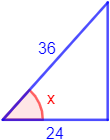
\includegraphics[scale=1]{P3.png}
\caption{Problema}
\end{figure}
la informacion que tenemos es hipotenusa y cateto adyacente, por lo que usaremos coseno:
\begin{align*}
    cos(x)&=\frac{24}{26}\\
    x=cos^{-1}(24/36)
\end{align*}
\begin{figure}[H]
\centering
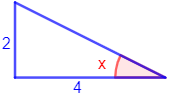
\includegraphics[scale=1]{P4.png}
\caption{Problema}
\end{figure}
tenemos informacion acerca de los dos catetos, asi que usaremos tangente:
\begin{align*}
    tan(x)&= \frac{2}{4}\\
    x&=arctan(2/4)
\end{align*}
\begin{figure}[H]
\centering
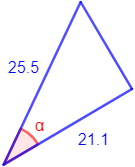
\includegraphics[scale=1]{P5.png}
\caption{Problema}
\end{figure}
tenemos informacion acerca de la hipotenusa y el cateto adyacente, por lo que usaremos coseno
\begin{align*}
    cos(\alpha)&= \frac{21.1}{25.5}\\
\alpha&= arccos(21.1/25.5)
\end{align*}
\begin{figure}[H]
\centering
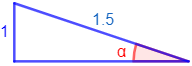
\includegraphics[scale=1]{P6.png}
\caption{Problema}
\end{figure}
tenemos informacion acerca del cateto opuesto y la hipotenusa, por lo que usaremos seno:
\begin{align*}
    sen(\alpha)&=\frac{1}{1.5}\\
    \alpha=arcsen(1/1.5)
\end{align*}
\begin{figure}[H]
\centering
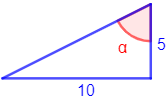
\includegraphics[scale=1]{P7.png}
\caption{Problema}
\end{figure}
tenemos informacion acerca del cateto opuesto y el cateto adyacente, por lo que usaremos tangente:
\begin{align*}
    tan(\alpha)=\frac{10}{5}\\
    \alpha=arctan(2)
\end{align*}
\begin{figure}[H]
\centering
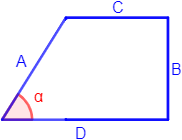
\includegraphics[scale=1]{P8.png}
\caption{Problema}
Calcular el área donde $\alpha=58$, B=C, A=24.6
\end{figure}
Aqui calcularemos el area del triangulo que puede ser formado junto con el rectangulo, calculando la altura del rectangulo tenemos que
\begin{align*}
    sen(\alpha)&= \frac{h}{24.6}\\
    h&=24.6sen(58)
\end{align*}
por lo que el área del triangulo es 
\begin{equation*}
    A_\Delta=\frac{(24.6sen(58)(24.6))}{2}
\end{equation*}
calculando el area del cuadrado tenemos que:
\begin{equation*}
    A_c=(24.6sen(58))^2
\end{equation*}
por lo que al final solo tenemos que sumar estas dos áreas
\end{document}